% To je predloga za poročila o domačih nalogah pri predmetih, katerih
% nosilec je Blaž Zupan. Seveda lahko tudi dodaš kakšen nov, zanimiv
% in uporaben element, ki ga v tej predlogi (še) ni. Več o LaTeX-u izveš na
% spletu, na primer na http://tobi.oetiker.ch/lshort/lshort.pdf.
%
% To predlogo lahko spremeniš v PDF dokument s pomočjo programa
% pdflatex, ki je del standardne instalacije LaTeX programov.

\documentclass[a4paper,11pt]{article}
\usepackage{a4wide}
\usepackage{fullpage}
\usepackage[utf8x]{inputenc}
\usepackage[slovene]{babel}
\selectlanguage{slovene}
\usepackage[toc,page]{appendix}
\usepackage[pdftex]{graphicx} % za slike
\usepackage{setspace}
\usepackage{color}
\definecolor{light-gray}{gray}{0.95}
\usepackage{listings} % za vključevanje kode
\usepackage{hyperref}
\usepackage{titlesec}

\renewcommand{\baselinestretch}{1.2} % za boljšo berljivost večji razmak
\renewcommand{\appendixpagename}{\normalfont\Large\bfseries{Priloge}}


\titleformat{name=\section}[runin]
  {\normalfont\bfseries}{}{0em}{}
\titleformat{name=\subsection}[runin]
  {\normalfont\bfseries}{}{0em}{}


% header
\makeatletter
\def\@maketitle{%
  \noindent
  \begin{minipage}{2in}
  \@author
  \end{minipage}
  \hfill
  \begin{minipage}{1.2in}
  \textbf{\@title}
  \end{minipage}
  \hfill
  \begin{minipage}{1.2in}
  \@date
  \end{minipage}
  \par
  \vskip 1.5em}
\makeatother


\lstset{ % nastavitve za izpis kode, sem lahko tudi kaj dodaš/spremeniš
language=Python,
basicstyle=\footnotesize,
basicstyle=\ttfamily\footnotesize\setstretch{1},
backgroundcolor=\color{light-gray},
}


% Naloga
\title{Naloga 2}
% Ime Priimek (vpisna)
\author{Andrej Hafner (63160122)}
\date{\today}

\begin{document}

\maketitle



\section{Izbrani jeziki}
Jeziki so bili izbrani tako, da so pokrivali zahtevane jezikovne skupine in da so bili čim bolj raznoliki in pisani v različnih abecedah. Vsi jeziki so evropski. Jeziki z abecedami, ki vsebujejo znake, ki niso kontekstno neodvisni (japonščina, kitajščina, korejščina) niso bili uporabljeni, saj jih Pythonova knjižnica \href{https://pypi.org/project/Unidecode/}{\it{unidecode}} slabo "prevede"  v osnovne ASCII znake. Izbrani romanski jeziki so italijanščina, francoščina, portugalščina, španščina in romunščina. Germanski jeziki so nemščina, danščina, švedščina, nizozemščina, angleščina, norveščina in islandščina. Slovanski jeziki so slovenščina, slovaščina, srbščina, ruščina, bulgarščina, češčina in polščina. Ostali jeziki so grščina, litvanščina, estonščina in turščina. Besedila so bila predobdelana tako, da je bil celoten tekst spremenjen v male znake abecede in pretvorjen iz posameznih abeced v osnovne ASCII znake z uporabo knjižnice \it{unidecode}.


\normalfont
\section{Rezultati razvrščanja}
Pri razvrščanju sta bili najslabša in najboljša porazdelitev izbrani na podlagi povprečne silhuete vseh držav. V primeru da je bila v gruči samo ena država, je le ta imela silhueto z vrednostjo 0. Pri najslabši porazdelitvi je imela povprečna silhueta vrednost 0.153, pri najboljši pa 0.287. Najboljše gruče so med seboj ločile slovanske, germanske in romanske jezike. V določenih gručah pride do vsiljicev, na primer angleščina med romanski jeziki. Jeziki, ki izrazito iztopajo pa se lahko celo pojavijo same v svoji gruči, na primer malteščina. Slabe gruče se oblikujejo kadar je bil medoid eden izmed iztopajočih jezikov.

\begin{figure}[htbp]
	\begin{center}
		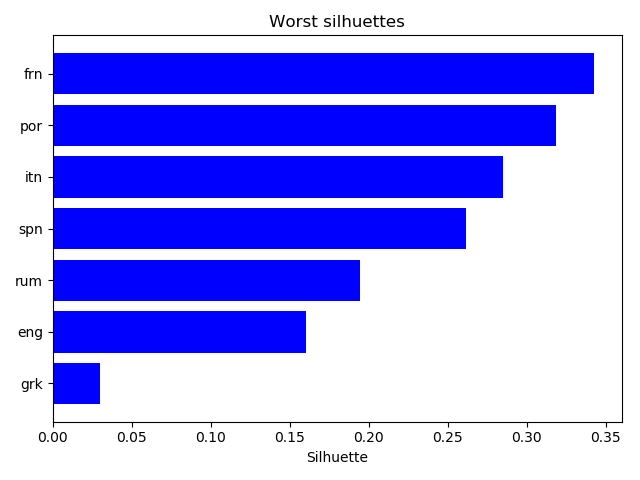
\includegraphics[scale=0.5]{worst1.png}
		\caption{Silhuete slabe gruče 1.}
		\label{slika1}
	\end{center}
\end{figure}

\begin{figure}[htbp]
	\begin{center}
		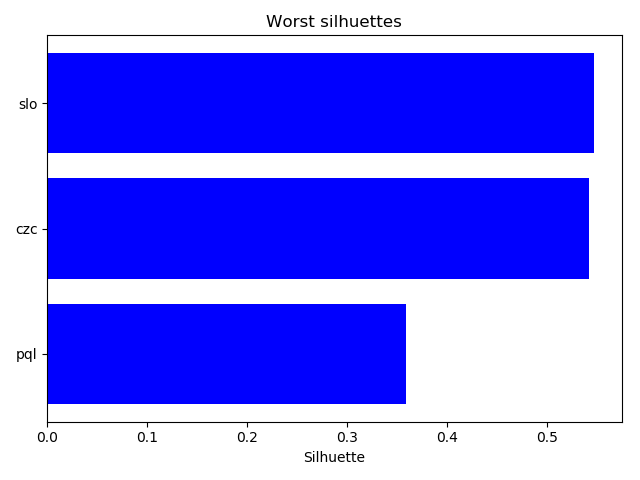
\includegraphics[scale=0.5]{worst2.png}
		\caption{Silhuete slabe gruče 2.}
		\label{slika1}
	\end{center}
\end{figure}

\begin{figure}[htbp]
	\begin{center}
		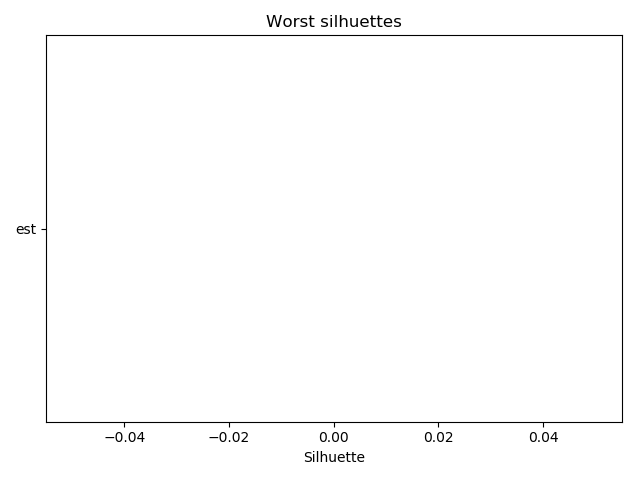
\includegraphics[scale=0.5]{worst3.png}
		\caption{Silhuete slabe gruče 3.}
		\label{slika1}
	\end{center}
\end{figure}

\begin{figure}[htbp]
	\begin{center}
		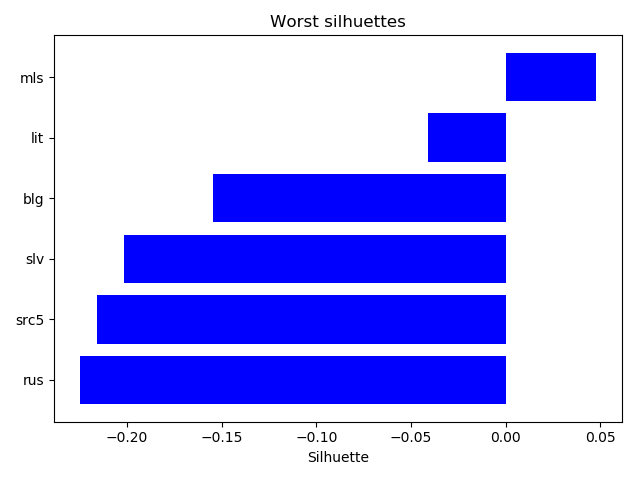
\includegraphics[scale=0.5]{worst4.png}
		\caption{Silhuete slabe gruče 4.}
		\label{slika1}
	\end{center}
\end{figure}

\begin{figure}[htbp]
	\begin{center}
		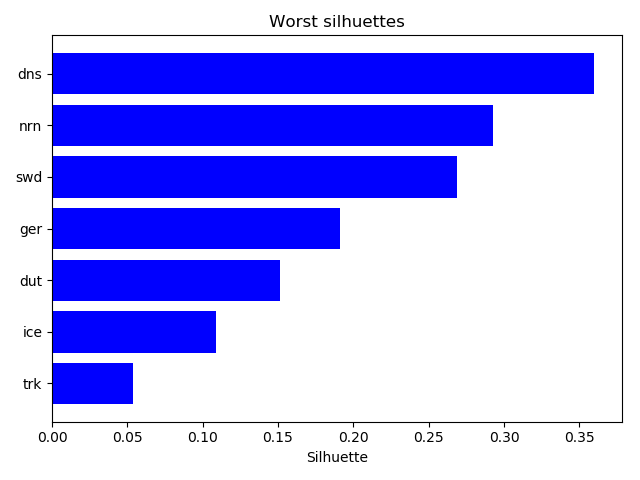
\includegraphics[scale=0.5]{worst5.png}
		\caption{Silhuete slabe gruče 5.}
		\label{slika1}
	\end{center}
\end{figure}

\begin{figure}[htbp]
	\begin{center}
		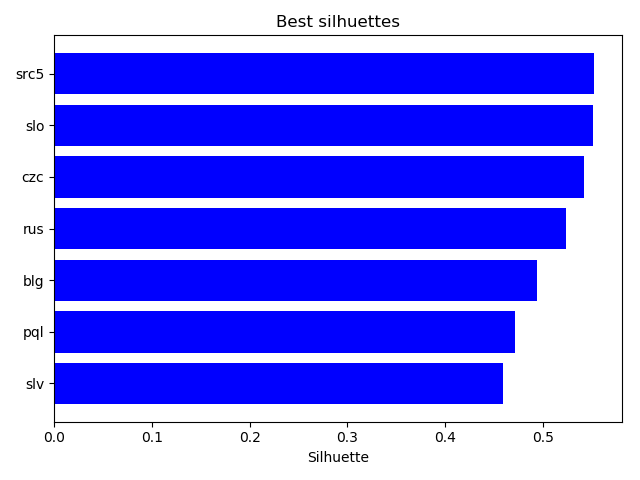
\includegraphics[scale=0.5]{best1.png}
		\caption{Silhuete dobre gruče 1 - slovanski jeziki.}
		\label{slika1}
	\end{center}
\end{figure}

\begin{figure}[htbp]
	\begin{center}
		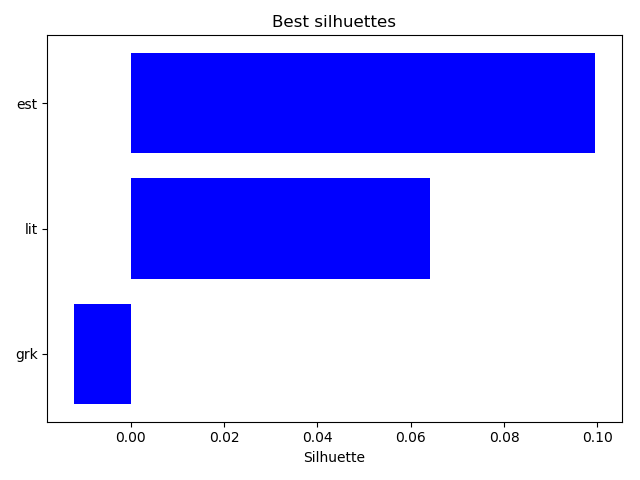
\includegraphics[scale=0.5]{best2.png}
		\caption{Silhuete dobre gruče 2 - baltska jezika z grščino, ki slabo pripada gruči.}
		\label{slika1}
	\end{center}
\end{figure}

\begin{figure}[htbp]
	\begin{center}
		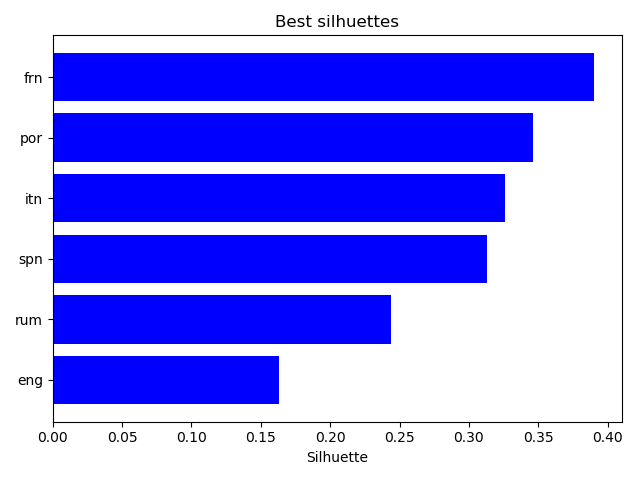
\includegraphics[scale=0.5]{best3.png}
		\caption{Silhuete dobre gruče 3 - romanski jeziki z izstopajočo angleščino.}
		\label{slika1}
	\end{center}
\end{figure}

\begin{figure}[htbp]
	\begin{center}
		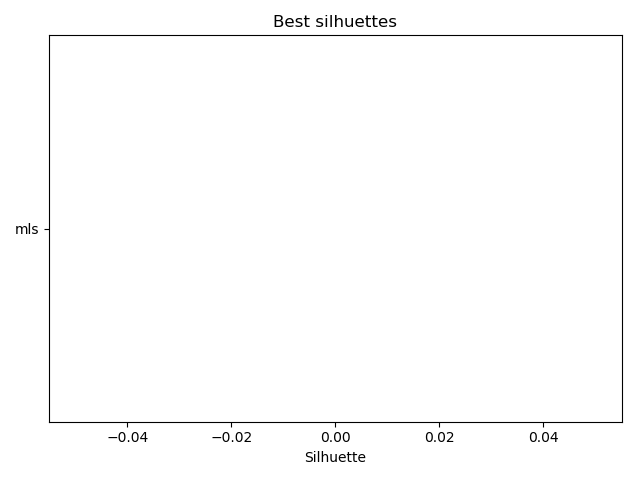
\includegraphics[scale=0.5]{best4.png}
		\caption{Silhuete dobre gruče 4.}
		\label{slika1}
	\end{center}
\end{figure}

\begin{figure}[htbp]
	\begin{center}
		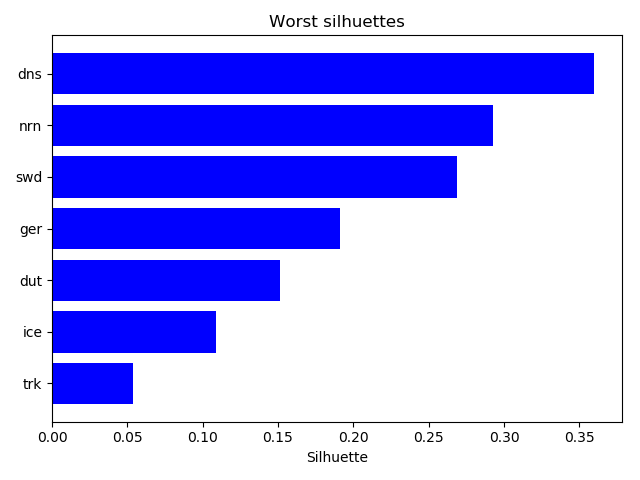
\includegraphics[scale=0.5]{worst5.png}
		\caption{Silhuete dobre gruče 5 - germanski jeziki z turščino.}
		\label{slika1}
	\end{center}
\end{figure}

\pagebreak
\section{Napovedovanje jezika}
Pri napovedi jezika se najprej izračuna frekvenca trojk za vse podane jezike, nato pa prav tako za podan odlomek. Sledi izračun kosinusne razdalje med frekvencami podanega teksta in frekvencami ostalih jezikov. Verjetnost se izračuna po formuli $p = 1 - razdalja$, nato pa se vzame tri jezike z največjimi verjetnostmi. 

\begin{table}[htbp]
	\caption{Tabela jezikov z odlomki in s kakšnimi verjetnostmi pripadajo najbolj verjetnim jezikom.}
	\label{tab1}
	\begin{center}
		\begin{tabular}{llp{3cm}}
			\hline
			jezik & tekst & najdene države in verjetnosti \\
			\hline
			švedščina & Kristerssons regering består av allt att döma av & švedščina - 0.67\\
			& hans eget parti och Kristdemokraterna. Men de två & islandščina - 0.61\\
			 & andra allianspartierna, Centern och Liberalerna, har tidigare & norveščina - 0.60\\
			 & sagt att man skulle rösta nej till M-ledarens så & \\
			 & kallade ”3–2–1”-regering, där inte alla partierna ingår. & \\
			 nemščina & Wie wird es nach den Midterm-Wahlen aussehen?& nemščina - 0.73 \\
			 & Viele Meinungsforscher und Medien versuchen, als  & norveščina - 0.69\\
			 & Reaktion auf die unzureichende Stimmungserfassung vor & svedščina - 0.67\\
			 & November 2016, neue Formen der Umfragen zu etablieren.  & \\
			 portugalščina & As novas orientações são bastante mais & portugalščina - 0.74\\
			 & rígidas do que as publicadas em 1998, quando os pais & litvanščina - 0.73\\ 
			 & eram aconselhados a desenvolver métodos alternativos à & ruščina - 0.63\\
			 & palmada em resposta a um comportamento indesejado. &  \\
			 češčina & To je vedle dalších podmínek nutné k tomu, & češčina - 0.63\\
			 & aby si mohli podat žádost o belgické občanství. & srbščina - 0.62\\
			 & Belgické orgány před rozsudkem žádost několika britských & polščina 0.62\\
			 & úředníků o udělení občanství odmítly. Zdůvodňovaly to tím, & \\
			 & že úředníci unijních institucí mají diplomatický status, & \\
			 & což znamená, že v zemi mimo jiné neplatí daň z příjmu, & \\
			 & která je v Belgii jedna z nejvyšších v Evropě. & \\
			\hline
		\end{tabular}
	\end{center}
\end{table}

\pagebreak

\section{Analiza izbranih novic}
Iz spleta so bile pobrane različne novice v 20 jezikih. Če nad njimi izvedemo razvrščanje na podlagi medoidov, so silhuete slabše, torej so tudi nastale gruče slabše. Najslabša povprečna silhueta je 0.103, najboljša pa 0.183, kar je za 0.104 manj od najboljše povprečne silhuete pri gručenju na podlagi deklaracij v različnih jezikih. Razlogov za to je več. Novice so krajše, med seboj se razlikujejo v dolžini in vsebina ni enaka. Vse to drži pri deklaraciji človekovih pravic.  

\section{Izjava o izdelavi domače naloge.}
Domačo nalogo in pripadajoče programe sem izdelal sam.


\end{document}
